\documentclass{article}

% Language setting
% Replace `english' with e.g. `spanish' to change the document language
\usepackage[english]{babel}
\usepackage{float} 

% Set page size and margins
% Replace `letterpaper' with `a4paper' for UK/EU standard size
\usepackage[letterpaper,top=2cm,bottom=2cm,left=3cm,right=3cm,marginparwidth=1.75cm]{geometry}
% Useful packages
\usepackage[round]{natbib}
\bibliographystyle{apalike}
\usepackage{amsmath}

\usepackage{graphicx}
\usepackage{subcaption}
\usepackage[colorlinks=true, allcolors=blue]{hyperref}

\title{\textbf{Correlation Analysis on Cryptocurrency and Traditional Financial Assets}}
\author{Yujie Tao
\\Zihan Liu
\\Wenqian Yang}

\begin{document}
\maketitle

\begin{abstract}
Currently, research on the dynamic relationship between cryptocurrency and traditional financial asset markets is limited and has yet to reach a consensus. This paper empirically examines the dynamic correlations among Bitcoin, the S\&P 500 Index, COMEX gold futures, and WTI crude oil futures within a unified framework, using daily trading data from November 2021, to January 2025.
This study tries to address a gap in existing research by systematically investigating the time-varying relationships between typical cryptocurrencies and traditional financial asset markets within a single framework. The study aims to improve the understanding of cryptocurrencies within modern financial assets and has significant implications for policymakers and investors alike.
\\
\textbf{Keywords}: cryptocurrency; financial assets; correlation analysis

\end{abstract}

\section{General View}

\

In general, bitcoin shows a moderate positive correlation with the S\&P 500 Index, while its relationships with COMEX Gold Futures and Aggregate Oil Futures are weaker and more variable. Traditional assets like gold and oil futures show a moderate positive correlation, reflecting shared macroeconomic influences.

In what follows in this report, we first compose a rather detailed literature review on the related topic and then display and explain some findings from our own research.
\section{Significance}
Due to the unique anonymity characteristics, cryptocurrencies are highly susceptible to asset price bubbles, and the contagion of such bubbles poses risks to the stability of the financial system. In fact, the anonymity of cryptocurrency users and the absence of intermediary institutions result in low transaction costs, making cryptocurrencies an attractive medium of exchange for potential users \cite{baur2018b}. However, cryptocurrencies are also characterized by high volatility \cite{chu2017,katsiampa2017}, heavy tails \cite{osterrieder2017,gkillas2018,phillip2018}, and leverage effects \cite{phillip2018}, distinguishing them as a new asset class rather than a traditional medium of exchange \cite{yermack2015,baek2015,dyhrberg2016b}. Many investors now view cryptocurrencies as alternative assets or diversification tools to reduce portfolio risk \cite{tiwari2019}. However, the cryptocurrency market remains less developed compared to traditional financial markets, and investor understanding of cryptocurrencies may not be entirely accurate. Consequently, the relationships between price volatility and risk spillovers between cryptocurrency and traditional financial markets are not yet fully understood.
This study’s examination of the correlation between cryptocurrency and traditional financial asset markets holds critical implications for policymakers and investors. Understanding the evolving relationship between cryptocurrencies and traditional financial assets can help policy makers formulate appropriate regulations to prevent contagion effects and protect financial stability. For investors, assessing the risk spillovers and hedging effectiveness of cryptocurrencies against traditional financial assets enables the selection of the most efficient cryptocurrency for hedging purposes and the evaluation of optimal hedging strategies.

\section{Literature Review}

\subsection{Studies on Price Volatility and Spillover Effects in the Cryptocurrency Market}
\cite{mensi2019cryptocurrency} use wavelet coherence and cross-wavelet transform methods to examine the interconnectedness among Bitcoin and five major cryptocurrencies (Dash, Ethereum, Litecoin, Monero, and Ripple) and the impact on portfolio risk. \cite{sifat2019} apply vector error correction models (VECM), Granger causality tests, autoregressive moving average (ARMA), and autoregressive distributed lag (ARDL) models to explore the leading and lagging price relationship between Bitcoin and Ethereum, concluding that they mutually influence each other. \cite{katsiampa2019} utilize diagonal BEKK and asymmetric diagonal BEKK models on intraday data of eight cryptocurrencies to investigate conditional volatility and covolatility among major cryptocurrencies, finding high volatility and strong interdependencies within the market.

\subsection{Studies on Price Volatility and Spillover Effects in Traditional Financial Markets}
\cite{mensi2021oil} analyze the spillover effects and correlations between crude oil futures and various maturities in the European Bond Market (EBM), further assessing the hedging effectiveness of oil-bond portfolios during calm and turbulent periods. \cite{sun2021spillover} examine spillover effects between the China oil and stock markets at different time frequencies based on the trading frequency, finding that the role of stocks as the main source of volatility varies across time domains. \cite{peng2020dynamic} employ linear and non-linear Granger causality tests in combination with bivariate empirical model decomposition to evaluate multi-scale dynamic interactions and volatility effects between the China stock market and the global oil market.

\subsection{Studies on Price Volatility and Spillover Effects Between Cryptocurrencies and Traditional Financial Markets}

Although various scholars have explored the dynamic relationship between cryptocurrencies and traditional financial assets, consensus remains elusive. \cite{dyhrberg2016b} find a strong correlation between cryptocurrency and stock markets. \cite{akyildirim2020relationship} identify a time-varying positive correlation between the conditional correlation of cryptocurrencies and financial market stress. They concluded that cryptocurrencies transmit risk to traditional financial assets, and different cryptocurrencies exhibit similar spillover patterns to traditional financial markets at specific times.

Conversely, \cite{corbet2019cryptocurrencies} and \cite{baur2018b} find that cryptocurrencies remain relatively isolated from traditional financial markets. \cite{baur2018b}, \cite{briere2015virtual}, and \cite{bouri2018bitcoin} argue that the correlation between cryptocurrencies and bonds or stocks is very low, suggesting that cryptocurrencies can serve as a diversification tool. Further studies by \cite{dyhrberg2016b}, \cite{bouri2018bitcoin}, and \cite{bencheikh2020asymmetric} demonstrate that cryptocurrencies exhibit some hedging capabilities relative to traditional financial assets. \cite{yermack2015} suggest that combining gold and Bitcoin can serve as a hedging strategy.

\


In summary, in the literature it is well recognized that cryptocurrencies and traditional financial asset markets exert impact on each other to various extents in terms of magnitude, the combination of both might help investors to diversify risks. 



\section{Data}


This study aims to investigate the relationship between the cryptocurrency market and traditional financial asset markets. For the cryptocurrency market, we initially considered the major cryptocurrencies with high market capitalization. To ensure data representativeness and continuity, we focused on cryptocurrencies with active trading and notable volatility between 2021 and 2024, including Bitcoin, Ethereum, and Ripple. After further screening, Bitcoin was chosen as the primary representative of the cryptocurrency market, as it has consistently maintained a dominant market share (more than 60\% of the total market capitalization) and its price trends tend to reflect broader market movements in cryptocurrency. This selection ensures both the representativeness of the study and avoids data issues that smaller or recently launched cryptocurrencies might present.

In terms of traditional financial assets, global oil prices currently refer to oil futures, with West Texas Intermediate (WTI) crude serving as a major global benchmark. The price movements of WTI often set the trend for other oil varieties. The US stock market, as one of the most influential capital markets worldwide, is represented by the S\&P 500 Index, which includes more than 500 publicly traded companies in various industries and is widely recognized as a suitable indicator of global stock market performance. Additionally, the gold futures market is a key component of the global financial market, and the COMEX gold futures, which are part of the New York Mercantile Exchange, are particularly influential, with the International Monetary Fund (IMF) and the US Treasury Department also trading on this exchange. COMEX gold futures often play a decisive role in global gold price trends. Consequently, this study uses the daily closing prices of the S\&P 500 Index, COMEX gold futures, and WTI crude oil futures to represent traditional financial asset market trends.
 
The data for this study cover daily closing prices from December 2021 to November 2024, totaling approximately 754 trading days.



To measure the daily returns of these assets, this study defines daily returns as the first-order logarithmic difference between closing prices on consecutive trading days. If $P_t$  represents the closing price at time t, then the daily return $Rt$ is defined as $R\_t = (\ln Pt - \ln P_{t-1}) \times 100\%$. 

\section{Results and Findings}





In this section, we report our main findings accompanied by some visualization figures.

\subsection{Correlation Analysis}




\begin{figure}[h!]
    \centering
    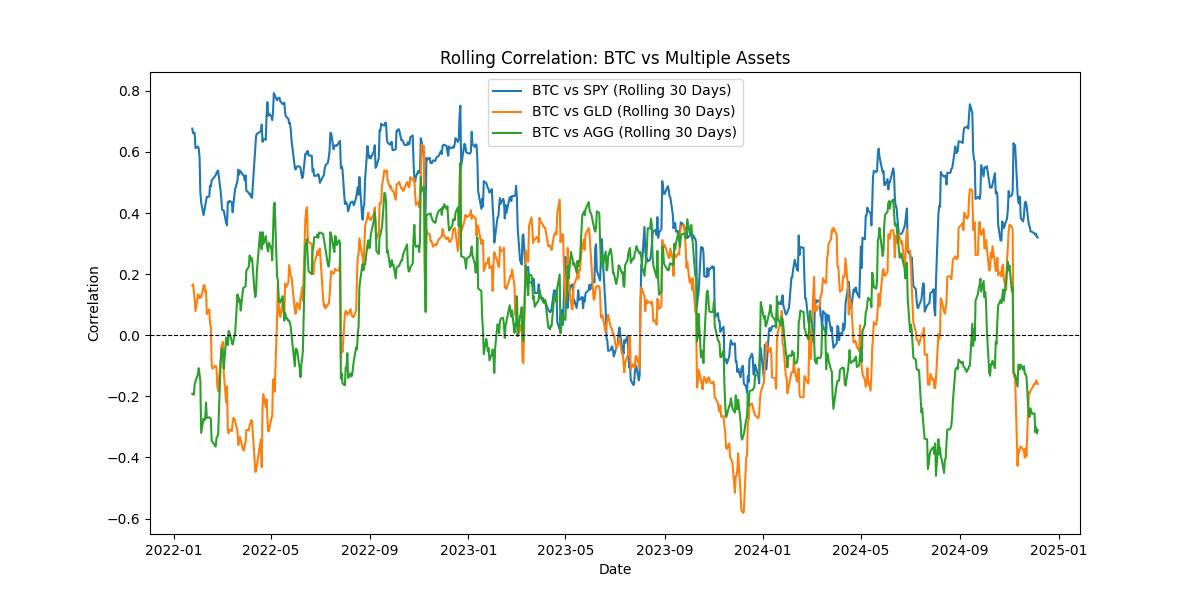
\includegraphics[width=0.8\textwidth]{src/models/results/rolling_correlation_multi.png}
    \caption{Correlation Analysis}
    \label{volatility}
    
\end{figure}


We analyze the correlations between Bitcoin and other major financial assets, focusing on both dynamic and static perspectives. Figure~\ref{volatility} illustrates the rolling 30-day correlation between Bitcoin and the S\&P 500 Index, COMEX Gold Futures and Aggregate Oil Futures from January 2022 to December 2024. Bitcoin’s correlation with the S\&P 500 Index remains predominantly positive, frequently ranging between 0.3 and 0.7, suggesting moderate alignment with equity markets and reflecting its behavior as a risky high-beta asset. Peaks near 0.7 indicate an increase in comovement, likely driven by macroeconomic events that affect both equities and cryptocurrencies. In contrast, the correlation of Bitcoin with COMEX Gold Futures shows substantial variability, oscillating between weakly negative and weakly positive values. Dips below -0.2 during early and late 2022 reflect instances where Bitcoin and gold likely acted as opposing risk hedges, while occasional positive correlations indicate alignment during broader economic shifts. The relationship of Bitcoin with aggregate oil futures is similarly inconsistent, with correlations fluctuating between -0.4 and 0.3, reflecting idiosyncratic shocks in the energy sector or the cryptocurrency market.

Figure~\ref{heat} further visualizes the pairwise correlations between different asset sectors. Among these, Bitcoin shows the strongest static correlation with the S\&P 500 Index (0.50), while its correlation with Gold Futures is weaker (0.17), highlighting Bitcoin’s unique speculative nature compared to the traditional role of gold as a safe haven. Similarly, Bitcoin exhibits a weak correlation with Oil Futures (0.16). Among traditional assets, Gold Futures and Oil Futures show a moderate positive correlation (0.48), likely driven by shared sensitivity to macroeconomic factors such as inflation and geopolitical risks. The general pattern underscores Bitcoin’s evolving role as both a speculative instrument and a potential diversification tool, influenced by macroeconomic trends, risk sentiment, and liquidity dynamics, while maintaining relative independence from commodities.

\begin{figure}[H]
    \centering
    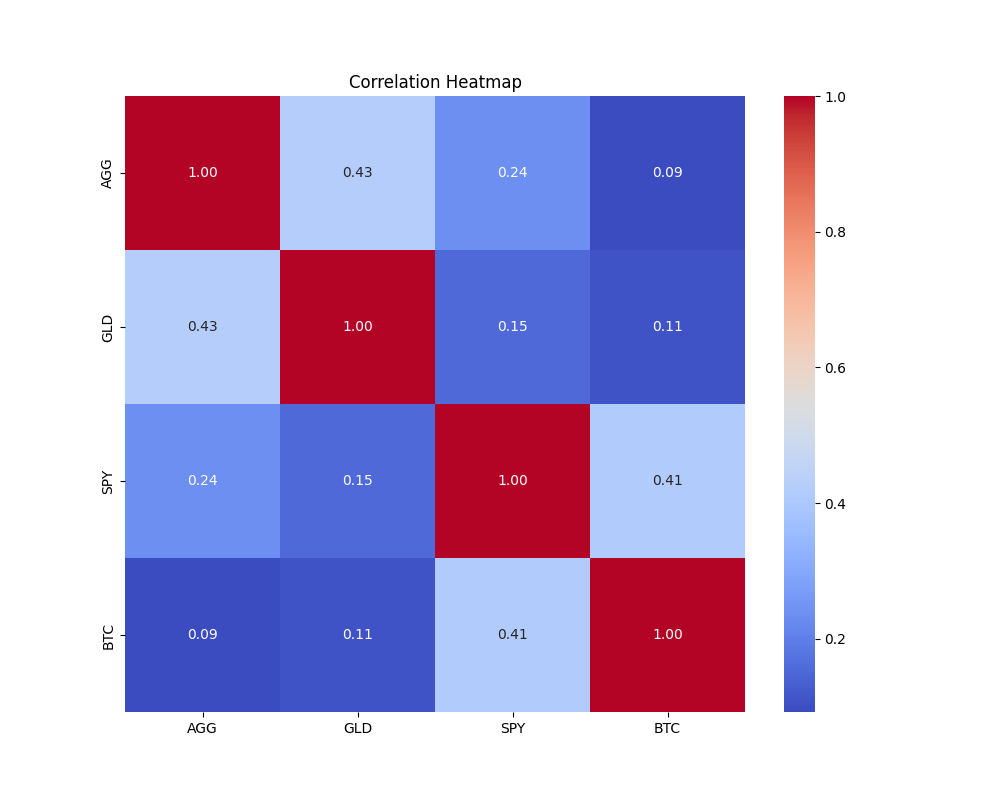
\includegraphics[width=0.5\textwidth]{src/models/results/correlation_heatmap.png}
    \caption{Correlation Heatmap}
    \label{heat}
    
\end{figure}
\

\subsection{Model}

In this section, we conduct Vector Autoregression Model and LSTM-based model to analyze and extract relationships between financial assets using time series data.

\subsubsection{Vector Autoregression Model}

The vector autoregression model (VAR) is particularly valuable in identifying how past movements in one asset influence the future dynamics of others. The graph displays the normalized daily closing prices of Bitcoin (BTC), the S\&P 500 Index (SPY), COMEX Gold Futures (GLD), and Aggregate Oil Futures (AGG), providing a comparative view of their dynamics over the study period.

\begin{figure}[h!]
    \centering
    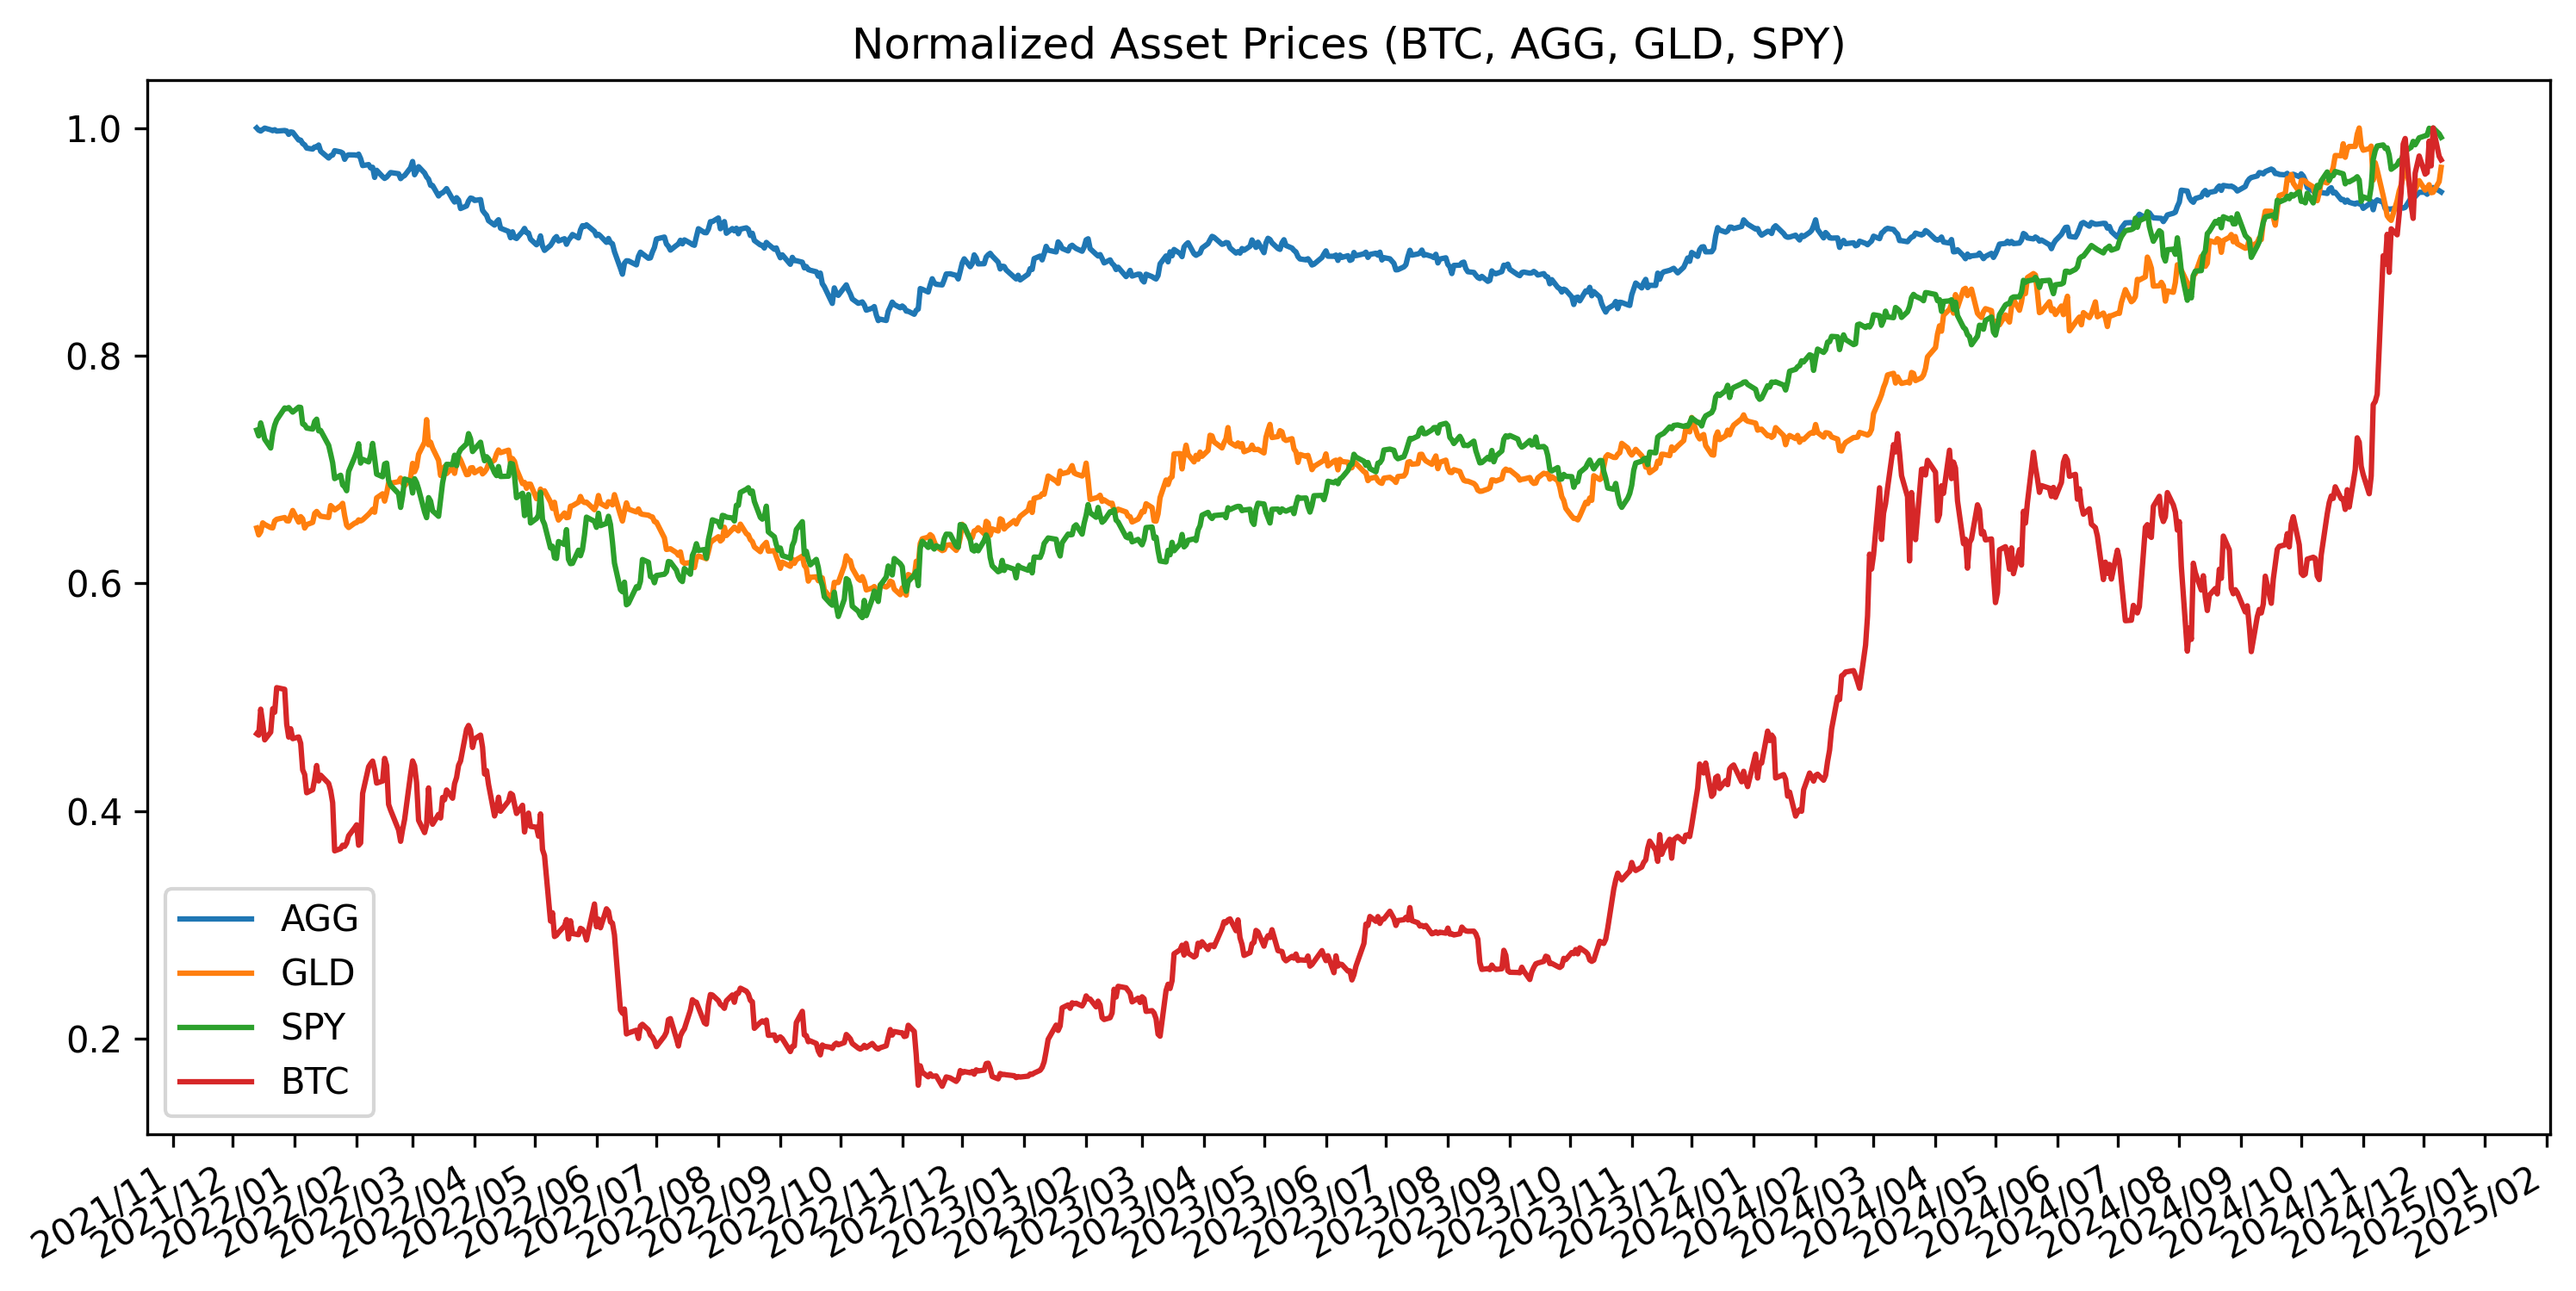
\includegraphics[width=0.8\textwidth]{src/models/results/normalized_asset_prices.png}
    \caption{Daily closing price time graphs for each asset}
    \label{prince}
    
\end{figure}

A notable observation is the significant volatility of Bitcoin, particularly during the period from 2024 to 2025, where sharp peaks and troughs reflect its highly speculative nature and susceptibility to market sentiment. This contrasts sharply with the relatively steady performance of S\&P 500 Index and the generally upward trends observed for COMEX Gold Futures and Aggregate Oil Futures, which align with the traditional roles of gold and oil as macroeconomically sensitive assets. The model also captures a stronger mutual influence between these traditional assets, reflecting their shared sensitivity to macroeconomic factors such as inflation, interest rate changes, and global economic conditions. 

 





\subsubsection{Long Short-Term Memory Model}





\begin{figure}[h!]
    \centering
    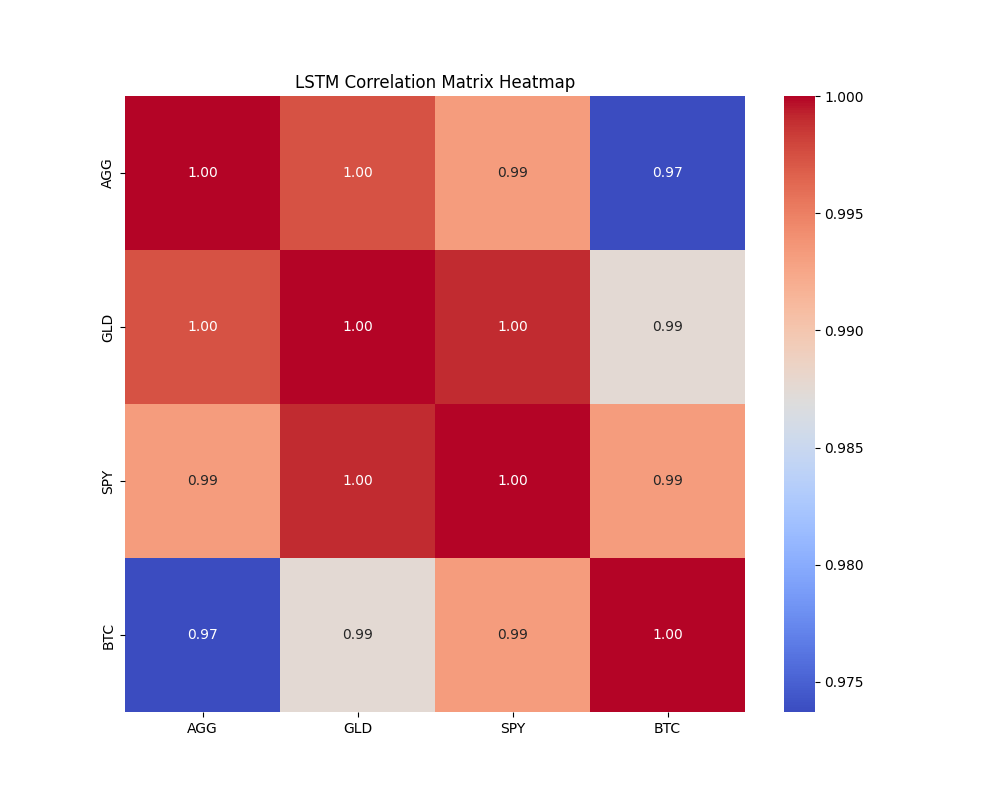
\includegraphics[width=0.5\textwidth]{src/models/results/lstm_correlation_heatmap_with_labels.png}
    \caption{LSTM Heatmap}
    \label{lstmh}
    
\end{figure}


Figure~\ref{lstmh} represents the heatmap of LSTM correlation matrix, revealing the relationships between the characteristics extracted by the model for the four financial assets. This matrix reveals different results from the other heatmap, the differences arise from their distinct methodologies. The Pearson correlation measures linear relationships based on historical data, ignoring time dependencies and non-linear dynamics. In contrast, the LSTM model processes data sequentially, capturing temporal dependencies, trends, and non-linear relationships that simple correlation cannot. Additionally, data transformations, such as scaling during LSTM training, can amplify correlations. However, improper tuning of the LSTM model can lead to overfitting and exaggerating relationships. These variations underscore the statistical simplicity of correlation analysis versus the complexity of LSTM’s temporal modeling. 

The matrix demonstrates an exceptionally high degree of correlation across all assets, with values close to or equal to 1. For example, Aggregate Oil Futures (AGG) and COMEX Gold Futures (GLD) exhibit a perfect correlation of 1.00, while Bitcoin (BTC) and the S\&P 500 Index (SPY) share a correlation of 0.99. This suggests that the model primarily captures systemic trends shared by these assets, such as responses to macroeconomic factors, rather than their unique individual characteristics. Interestingly, Bitcoin, which is often perceived as less correlated with traditional assets, also displays high correlations, indicating that the model may be emphasizing broader market dynamics such as liquidity or sentiment shifts.


In conclusion, while the correlation heatmap indicates that the LSTM model successfully identifies shared market dynamics among the assets, the lack of differentiation in correlations highlights a potential limitation in capturing asset-specific nuances. However, the training loss curve confirms the strong learning efficiency and convergence of the model, suggesting its robustness in handling time-series data. Future work could focus on refining the model to better isolate unique asset behaviors while maintaining its ability to capture systemic relationships.

\section{Conclusion}


This study provides an empirical analysis of the dynamic relationships between Bitcoin and traditional financial assets, including the S\&P 500 Index, COMEX Gold Futures, and WTI Crude Oil Futures. By leveraging both traditional Pearson correlation analysis and an LSTM-based modeling approach, we uncover distinct insights into the interdependencies among these assets. The Pearson correlation analysis highlights the linear relationships, revealing that Bitcoin demonstrates moderate positive correlations with the S\&P 500 Index but weaker and more variable connections with Gold and Oil Futures. These findings reflect Bitcoin’s evolving role as a speculative asset and its occasional behavior as a diversification tool. Var model shows that Bitcoin exhibits a highly volatile and speculative nature, showing weaker and less consistent correlations with traditional assets like the \S&P 500, gold, and oil, which are more influenced by macroeconomic factors and exhibit stable, predictable trends.
However, the LSTM-based correlation heatmap reveals stronger correlations across all assets, suggesting that the model captures shared systemic dynamics, such as responses to macroeconomic factors, liquidity conditions, and market sentiment shifts. While the LSTM model effectively identifies broader market trends and temporal dependencies, it appears less adept at isolating the unique characteristics of individual assets, potentially due to overfitting or the inherent nature of data preprocessing.

This study highlights the importance of combining traditional statistical approaches with advanced machine learning models to gain a comprehensive understanding of asset relationships. However, the results underscore the need for caution when interpreting model-driven correlations, as they may amplify relationships influenced by data transformations or systemic trends. Future research could refine the LSTM model to better differentiate asset-specific behaviors while maintaining its strength in capturing complex temporal and non-linear relationships. These findings provide valuable implications for policy makers and investors, providing insight into risk management, hedging strategies, and the evolving interplay between cryptocurrencies and traditional financial markets.



\newpage
\bibliographystyle{plain}
\bibliography{Bibliography}
\end{document}
